\chapter{Chapter/Section Topics and Sequence}
\label{ch:roadmap}

Formulas and equations provide a foundation
underlying most of the topics
discussed in this text.
A stream of formalism underlies the presentation of classical logic
and reasoning about digital circuits and computer programs.
Parts of the discussion that focus
on large-scale computation takes a more descriptive approach,
and these parts can be woven into a study of the material
at any point. There are some other places, too, where
sections can be studied out of sequence.
The following diagram elucidates some options.
\vspace{1cm}
\label{diagram:roadmap}
\begin{center}
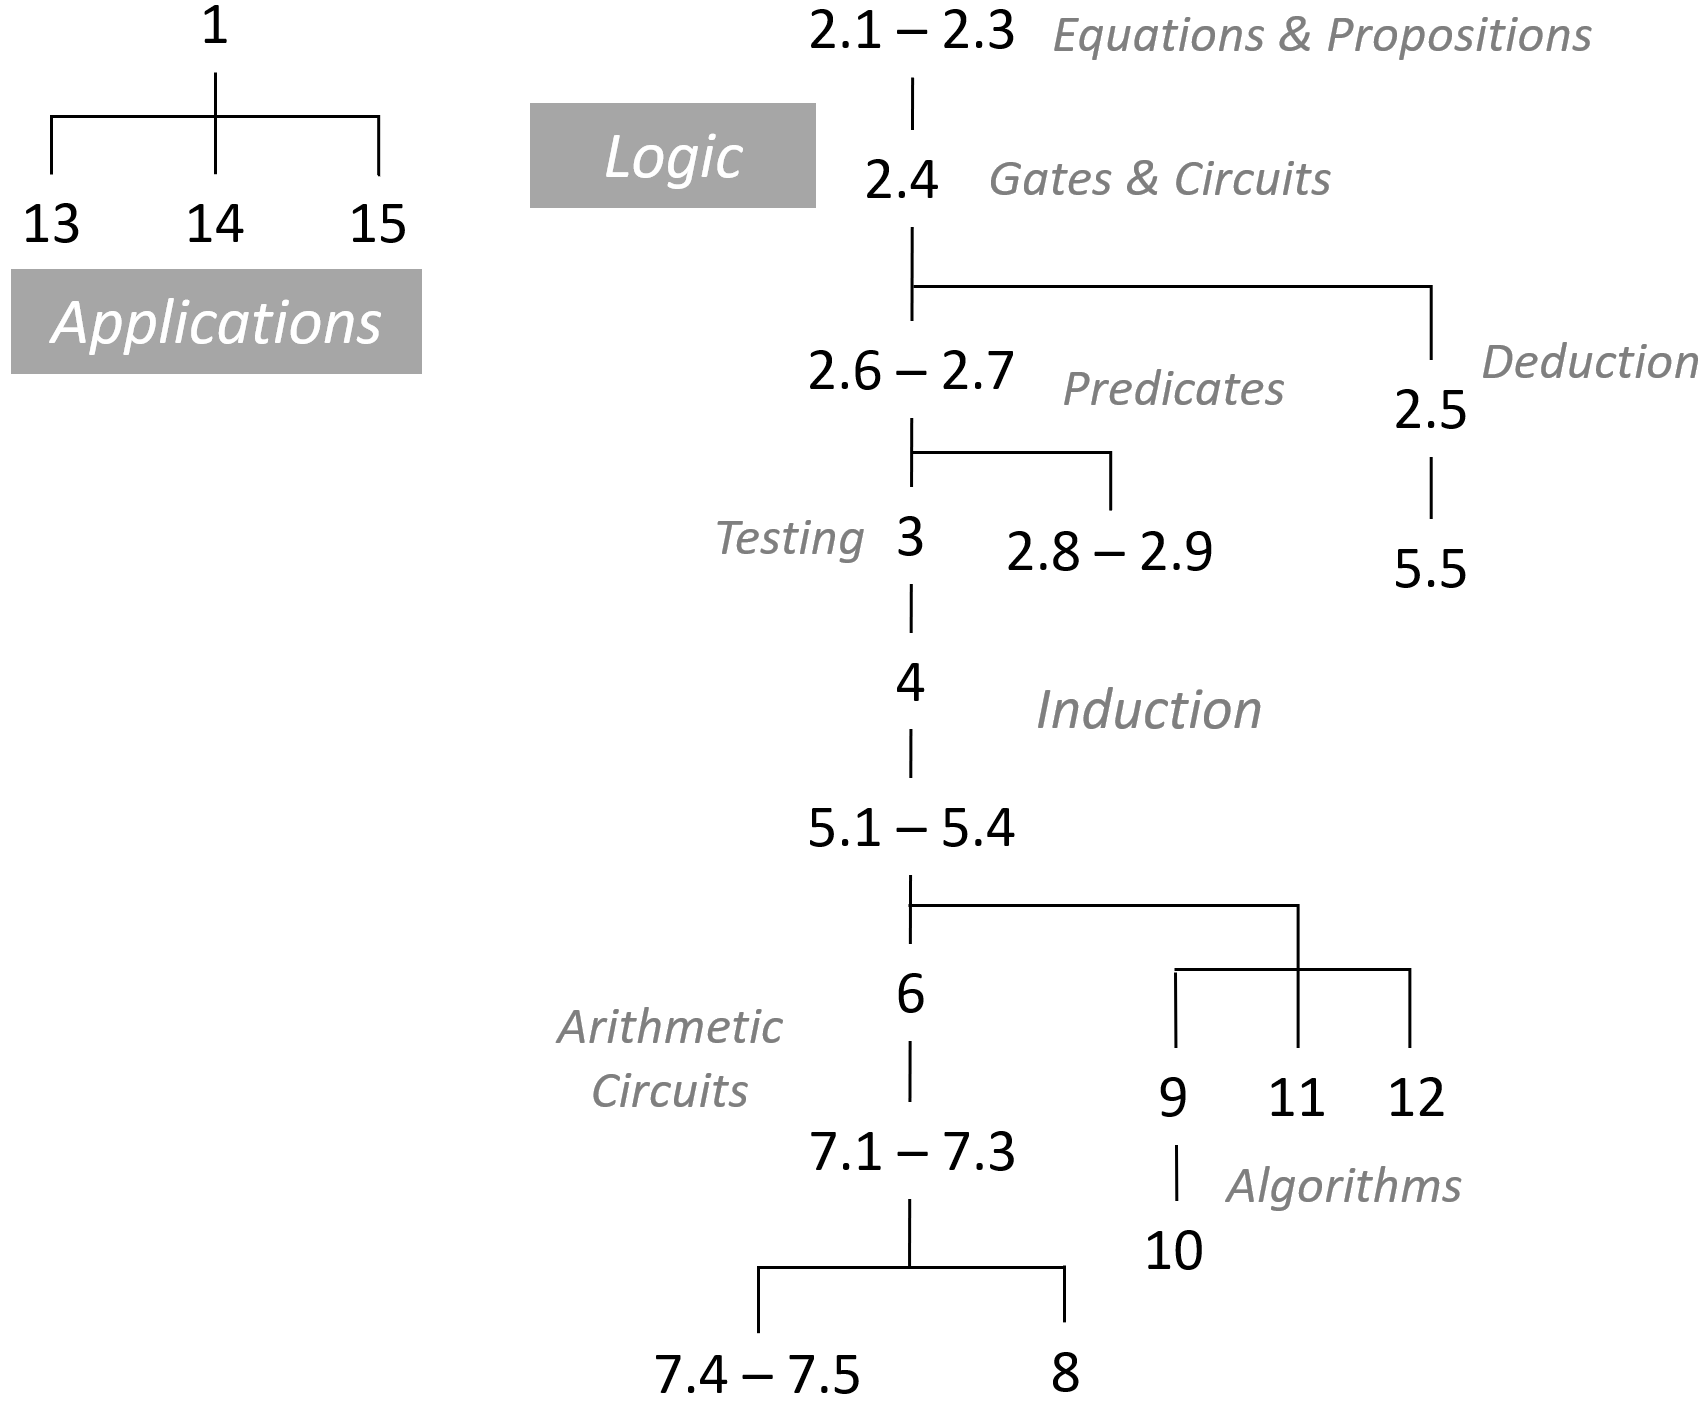
\includegraphics[scale=0.25]{images/roadmap.png}
\end{center}


%%% Local Variables:
%%% mode: latex
%%% TeX-master: "book"
%%% End:
